\section{Laboratory work implementation}

\subsection{Tasks and Points}
\begin{itemize}
	\item Basic Level (nota 5 || 6):
	
	\item Normal Level (nota 7 || 8):
	
	\item Advanced Level (nota 9 || 10):
	Dezvoltarea unei aplicatii: 
	\begin{itemize}
		\item Desktop
    	\item Mobile	
    	\item Web
    	\item Browser Extension
    	\item Game Development(web,mobile,desktop)
    	\item Service Application
    	\item Internet Application
    	\item Client Application
	\end{itemize}
\end{itemize}
    



\subsection{Analiza lucrarii de laborator}

Linkul la repozitorul Github:\\
\begin{center}
\url{https://github.com/dmitrii724/MIDPS}
\end{center}

Pentru a realiza acest proiect am utilizat Unity deoarece ne permite posibilitatea de crea aplicatii cross-platform cu usurinta doar avind compnentele necesare instalate pentru platforma dorita.Acest proiect a fost realizat pentru Android si anume Windows(De la versiunea 4.0.1).
\begin{center}
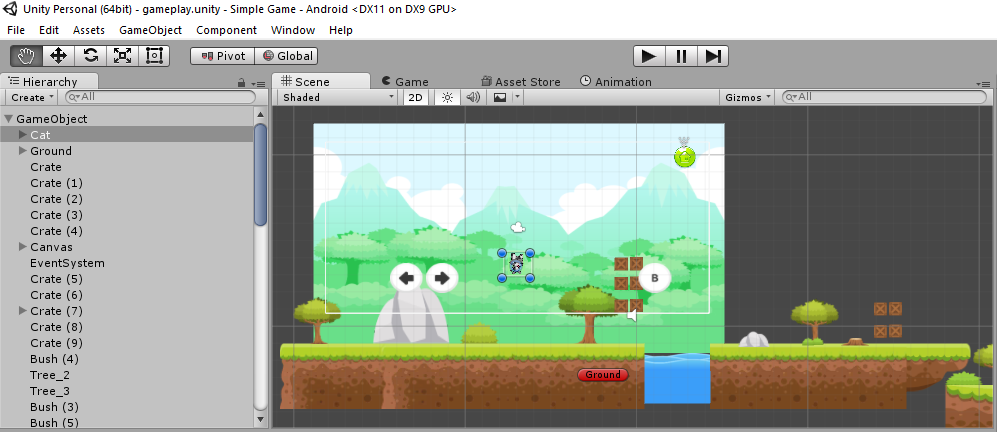
\includegraphics[scale=0.5]{images/1}
\end{center}

Deoarece acest proiect trebuia de realizat in grup ,pentru aceasta ma divizat task-urile in felul urmator:\\
-Colegul meu de proiect face coding-ul si combinarea tutror compnentelor in Unity pentru a primi rezultatul final.\\
-Eu fac meniul pentru joc si raspund de crearea si gasirea modelelor 2D,imaginile 2D ,Sunetul,Scena.\\

Pentru inceput am gasit modele 2D (imagini) ale Motanului pentru joc. Am gasit mai multe imagini cu Pisica data pentru ca in pasii urmatori colegul meu de proiect sa elaboreze animatie la miscarea pisicii pe scenele elaborate de mine.
\begin{center}
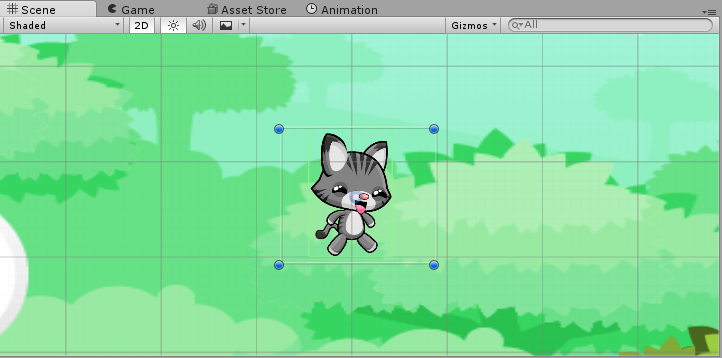
\includegraphics[scale=1]{images/cat}
\end{center}

Partea a doua a task-ului meu a fost elaborarea scenei principale ale jocului. In elaborarea acestui punct, am unit detaliile modelelor 2D in niste imagini mai detailate.
\begin{center}
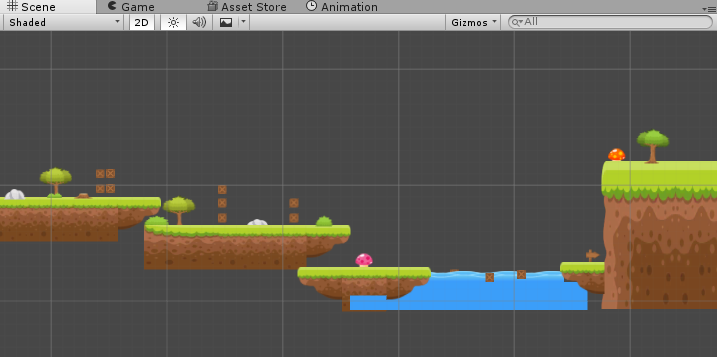
\includegraphics[scale=1]{images/ground}
\end{center}

Am elaborat meniul jocului cu butonul necesar pentru a porni joaca "Play".
\begin{center}
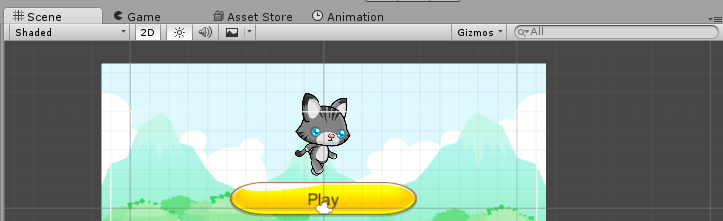
\includegraphics[scale=1]{images/menu}\\
\end{center}

De asemenea am elaborat si un meniu cu un mesaj pentru sfirsitul jocului in cazul trecerii cu succes a nivelului.
\begin{center}
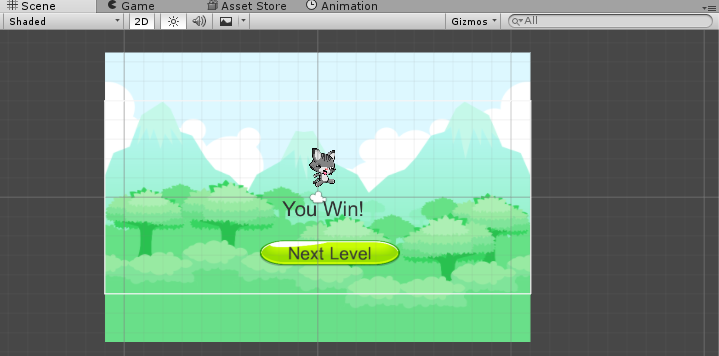
\includegraphics[scale=1]{images/win}\\
\end{center}
\clearpage